\documentclass[a4paper,12pt]{article}
\usepackage{graphicx} % Required for inserting images
\usepackage{color}
\usepackage[UTF8]{ctex}
\usepackage{amsmath}
\usepackage{tabularray}



%\newcommand{\upsite}[1]{\textsuperscript}{cite{#1}}

%\bibliographystyle{unsrt}
\begin{document}
\begin{figure}[t]
    
\includegraphics[width=0.5\textwidth]{ouc2.png}
\end{figure}

\title{\textbf{实验报告}}
\author{单衍喆 }
\date{2024-9-14}
\maketitle

\pagenumbering{roman}
\text{GitHub地址:https://github.com/Venusss1/course.git}

\newpage
\begin{figure}[t]
    
\includegraphics[width=0.2\textwidth]{ouc.jpg}
\end{figure}

\tableofcontents
\newpage
\pagenumbering{arabic}


\section{\underline{\color{blue}实验内容}}

\begin{enumerate}
    \item \textbf{调试及性能分析}
    \item \textbf{元编程}
    \item \textbf{大杂烩}
    \item \textbf{pytorch应用}
\end{enumerate}

\section{\underline{\color{blue}实验设计}}

\subsection{\color{red}调试及性能分析}
\subsubsection{\color{green}gdb调试c语言及c++程序}
\begin{enumerate}
    \item 编译可执行程序
    \item 启动gdb
    \begin{figure}[h]
        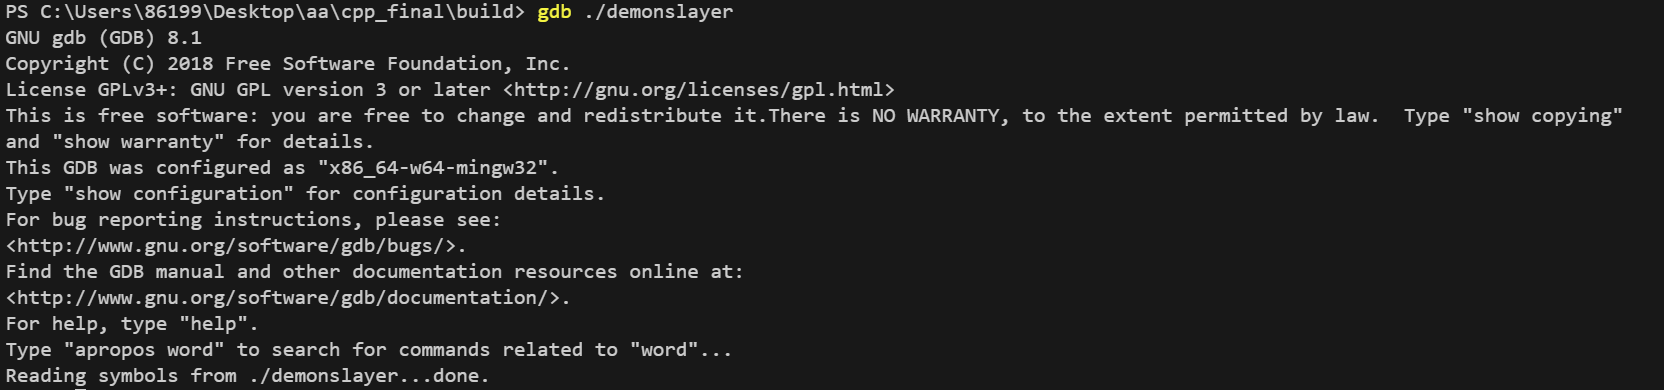
\includegraphics[width=1\textwidth]{gdb.png}
        \caption{启动gdb}
    \end{figure}
    \item 设置断点
    \item gdb调试程序
\end{enumerate}

\newpage
\subsubsection{\color{green}基本命令}
\begin{table}[h]
\centering
\caption{基本命令}
\begin{tabular}{|l|l|l|} 
\hline
\multicolumn{1}{|c|}{简写} & \multicolumn{1}{c|}{全称} & \multicolumn{1}{c|}{作用}  \\ 
\hline
b                        & break                   & 设置断点                     \\ 
\hline
r                        & run                     & 运行程序                     \\ 
\hline
n                        & next                    & 继续执行                     \\ 
\hline
f                        & finish                  & 结束当前函数                   \\ 
\hline
c                        & continue                & 继续运行程序                   \\ 
\hline
p                        & print                   & 打印                       \\
\hline
\end{tabular}
\end{table}



\subsection{\color{red}元编程}
\subsubsection{\color{green}Cmake构建流程}
\begin{enumerate}
    \item 确定构建目录:\\“Out-of-source”,构建文件放在源代码目录之外的独立目录中
    \item 使用CMake生成构建文件:
    \begin{verbatim}
        CMake -DCMAKE_BUILD\_TYPE=Release ..
    \end{verbatim}
    \item 编译和构建:
    \begin{verbatim}
        make <your_project_name>
    \end{verbatim}
    \item 清理构建文件:
    \begin{verbatim}
        make clean
    \end{verbatim}
\end{enumerate}
\subsubsection{\color{green}Cmake构建项目}
\begin{itemize}
    \item 规定最低的版本:
    \begin{verbatim}
        cmake minimum required(VERSION 3.12)
    \end{verbatim}
    \item 构建项目名称: 
    \begin{verbatim}
        project(cpp final)
    \end{verbatim}
    \item 设置变量:
    \begin{verbatim}
        set(mainTargetName  "demonslayer"\)
    \end{verbatim}
    \item 自定义命令:
    \begin{verbatim}
        add_custom_command(
        <type> <name> <COMMAND> <WORKING_DIRECTORY> <OUTPUT> <DEPENDS>
        [<VERBOSE>]
        [<COMMENT>]
)
    \end{verbatim}
    \item 迭代:
    \begin{verbatim}
        foreach(<var> <item> <condition>)
            <statement>
        endforeach()
    \end{verbatim}
\end{itemize}
\subsubsection{\color{green}makefile基本语法}
\begin{itemize}
    \item 编译命令:
    \begin{verbatim}
        hello.c main.c test.c
            gcc main.c test.c
    \end{verbatim}
    \item 目标文件
    \begin{verbatim}
        main.o: main.c
            gcc -c main.c
    \end{verbatim}
    \item 伪命令
    \begin{verbatim}
        .PHONY:clean
        clean:
            rm -f *.o hello
    \end{verbatim}
    \item 变量\\ $targets = hello $
\end{itemize}

\subsection{\color{red}大杂烩}
\subsubsection{\color{green}修改键位映射}
使用AutoHotKey修改键位映射
\begin{enumerate}
    \item 下载安装AutoHotKey
    \begin{figure}[h]
        \centering
        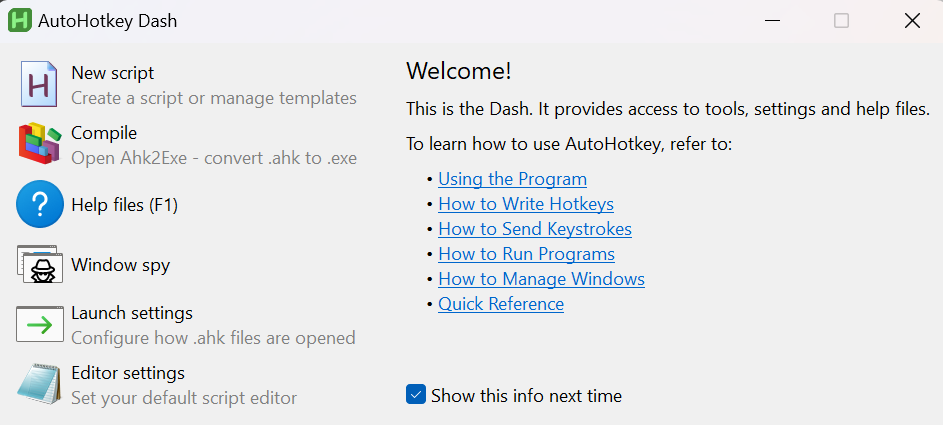
\includegraphics[width=0.5\textwidth]{board.png}
        \caption{autoHotKey}
    \end{figure}
    \item 配置脚本文件:交换将capslock大写锁定键映射到esc
    \item 运行脚本文件
    \item 配置开机启动项
\end{enumerate}
\subsubsection{\color{green}MarkDown纯文本编辑}
\begin{itemize}
    \item 标题
        \begin{verbatim}
            # 标题1
            ## 标题2
        \end{verbatim}
    \item 段落
    \begin{verbatim}
        <p>
        这是一个段落。
        <p>
    \end{verbatim}
    \item 链接
    \begin{verbatim}
        <a href="URL">链接文字</a>
    \end{verbatim}
    \item 图片
    \begin{verbatim}
        <img src="URL" alt="图片描述" />
    \end{verbatim}
    \item 代码块
    \begin{verbatim}
        <pre>
        <code>
        这是一些代码。
        </code>
        </pre>
    \end{verbatim}
\end{itemize}



\subsubsection{\color{green}vpn}
\begin{enumerate}
    \item 下载安装clash for windows
    \begin{figure}[h]
        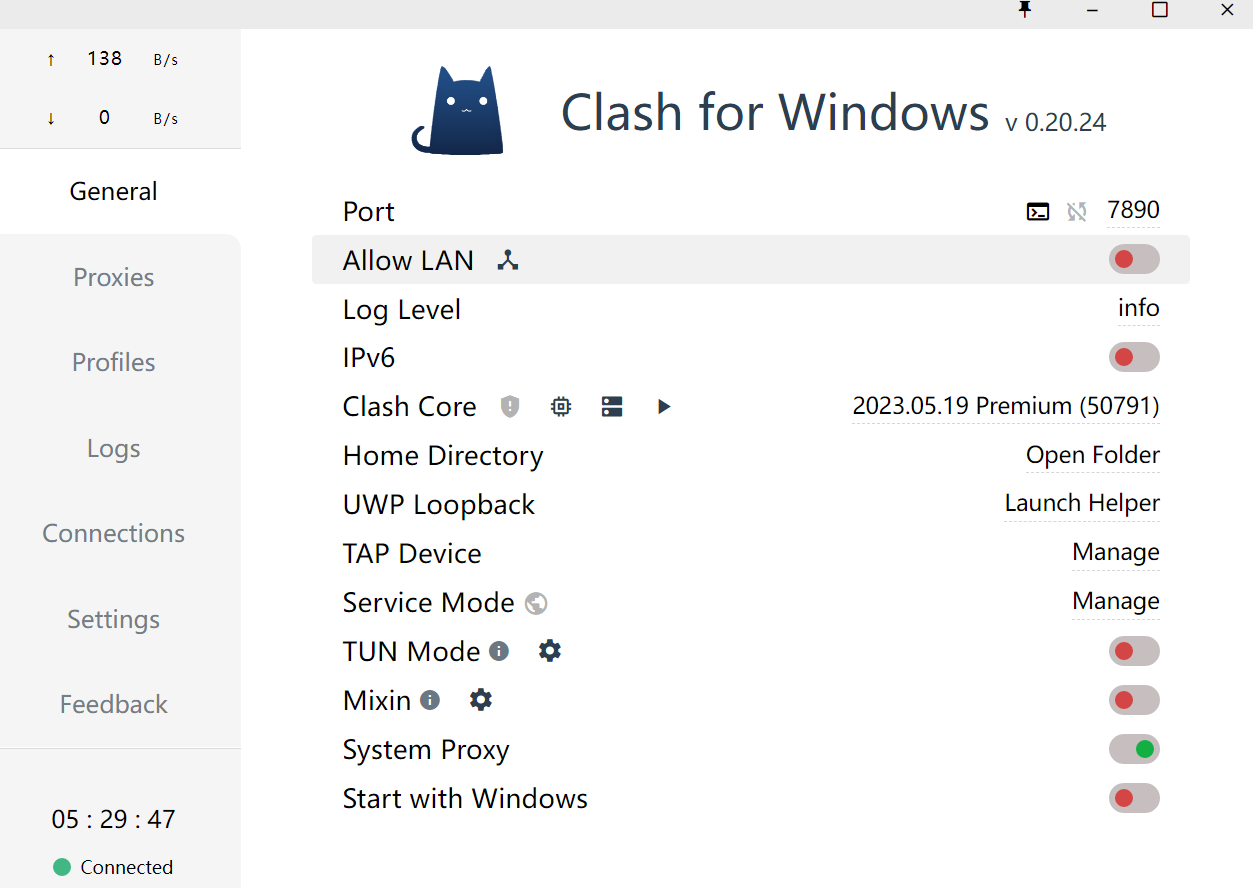
\includegraphics[width=0.5\textwidth]{vpn.png}
        \caption{clash for windows}      
    \end{figure}
    \item 配置profiles
    \item 打开system Proxy
\end{enumerate}


\subsection{\color{red}pytorch应用}
    \subsubsection{\color{green}transform} 
    帮助用户在训练和推理过程中对数据进行预处理、数据增强、数据转换等操作
        \begin{verbatim}
            data_transform = {
                "train": transforms.Compose([transforms.RandomResizedCrop(224),
                                            transforms.RandomHorizontalFlip(),
                                            transforms.ToTensor(),
                                            transforms.Normalize([0.485, 0.456, 0.406], [0.229, 0.224, 0.225])]),
                "val": transforms.Compose([transforms.Resize(256),
                                        transforms.CenterCrop(224),
                                        transforms.ToTensor(),
                                        transforms.Normalize([0.485, 0.456, 0.406], [0.229, 0.224, 0.225])])}
        \end{verbatim}

    \subsubsection{\color{green}DataLoader} 
    帮助用户自动加载训练数据,并行处理数据,以及控制数据读取的速度和策略
        \begin{verbatim}
                train_loader = torch.utils.data.DataLoader(train_dataset,
                                            batch_size=batch_size, shuffle=True,
                                            num_workers=nw)
        \end{verbatim}

    \subsubsection{\color{green}train epoch} 
    核心循环
        \begin{verbatim}
            epochs = 3
            best_acc = 0.0
            save_path = './resNet34.pth'
            train_steps = len(train_loader)
            for epoch in range(epochs):
                net.train()
                running_loss = 0.0
                train_bar = tqdm(train_loader, file=sys.stdout)

                for step, data in enumerate(train_bar):
                    images, labels = data
                    optimizer.zero_grad()
                    logits = net(images.to(device))
                    loss = loss_function(logits, labels.to(device))
                    loss.backward()
                    optimizer.step()

                    running_loss += loss.item()

        \end{verbatim}

    \subsubsection{\color{green}loss function} 
    用于衡量模型预测和真实值之间的差距
            \begin{itemize}
                \item MSE(均方误差)
            \begin{verbatim}
                def mse_loss(y_true, y_pred):
                return np.mean((y_true - y_pred) ** 2, axis=1)
            \end{verbatim}
                \item Cross-Entropy(交叉熵)
            \begin{verbatim}
                def cross_entropy_loss(y_true, y_pred):
                return -np.sum(np.log(y_pred) * y_true, axis=1)
            \end{verbatim}
            \end{itemize}

    \subsubsection{\color{green}optimizer}
    用于最小化损失函数,从而实现模型的训练和优化
            \begin{itemize}
            \item Adam(自适应矩阵梯度下降)
            \begin{verbatim}
                def adam(params, grads, lr=0.001, beta1=0.9, beta2=0.999, epsilon=1e-8):
                m = params.data.mean()
                v = params.grad.data.mean()
                for i in range(params.size):
                    m_hat = beta1 * m + (1 - beta1) * params.data[i]
                    v_hat = beta2 * v + (1 - beta2) * grads.data[i]
                    params.data[i] = -lr * m_hat / (np.sqrt(v_hat) + epsilon)
                    v[i] = beta2 * v_hat
                return params
                    \end{verbatim}
                \item SGD(随机梯度下降)
            \begin{verbatim}
                def adam(params, grads, lr=0.001, beta1=0.9, beta2=0.999, epsilon=1e-8):
                m = params.data.mean()
                v = params.grad.data.mean()
                for i in range(params.size):
                    m_hat = beta1 * m + (1 - beta1) * params.data[i]
                    v_hat = beta2 * v + (1 - beta2) * grads.data[i]
                    params.data[i] = -lr * m_hat / (np.sqrt(v_hat) + epsilon)
                    v[i] = beta2 * v_hat
                return params
            \end{verbatim}
            \end{itemize}


\newpage
\section{\underline{\color{blue}实验心得}}
通过本次实验,我学会了运用pytorch进行深度学习的基本步骤和基本参数的设置,为之后人工智能的学习打下基础;\\
我学会了用gdb调试c语言及c++代码的基本步骤,学会了用gdb调试寻找代码问题;\\
了解了CMake构建项目的基本流程及CMake的基本命令,学会了makefile的基本语法;\\
学会了许多和计算机有关的知识,包括键盘映射,vpn网络设置,GitHub的使用及纯文本编辑工具Markdown。


\end{document}
